\documentclass[twocolumn]{ctexbook}

\usepackage{chemfig}
\usepackage{float}
\usepackage{natbib}
\usepackage{ctex}
\usepackage{url}
\usepackage{framed}
\usepackage{graphicx}
\usepackage{setspace}
\usepackage{enumerate}
\usepackage[final]{pdfpages}
\usepackage{threeparttable}
\usepackage{booktabs}
\usepackage{hyperref}
\usepackage{hyperxmp}

\usepackage{minipage-marginpar}
\usepackage{subfigure}
\graphicspath{{fig/}}

\hypersetup{pdfinfo={
Author = {苏靖云, 戚鉴清, 石强, 皇甫硕龙, 白雪杨},
Title = {国内制药企业在不同发展模式下的创新能力与出路},
Subject = Draft version,
Keywords = {制药, 创新, 研发外包, 合作},},
pdfcopyright = {Copyright (C) 2019 by Jian-Qing Qi.
	All rights reserved.},
pdflicenseurl = {wxid:graphicx}}


\title{\textbf{国内制药企业在不同发展模式下的创新能力与出路}\\{\textit{“药创未来”支队调研报告}}}


	%etitle = {A Preliminary Research on the Innovation Capability of Domestic Pharmaceutical Companies},



\author{苏靖云,戚鉴清,石强,皇甫硕龙,白雪杨}
	%eauthor = {Jing-Yun Su, Jian-Qing Qi, Qiang Shi, Shuo-Long Huang-Fu, Xue-Yang Bai},


\bibliographystyle{apalike}


\begin{document}

\frontmatter
\onecolumn
\includepdf[pages=1]{fig/cover4.pdf}
\begin{spacing}{2.0}
\chapter{摘要}
	

	


	在我国强调创新的环境下,新药研发逐渐成为制药企业竞争的核心,不同发展模式的企业做出了不同的抉择。文章以三家企业为对象,通过对其研发模式、合作方式、人员组成的调研及国家政策的概括,分析其创新能力与出路。结果表明,由于部分小型企业自身研发能力不足,目前仍有企业坚持只进行仿制,大部分企业逐渐向新药研发转型,同时也出现了进行CMO/CDMO服务的企业。在这样的背景下,进行多样化的企业间合作,以及对医药领域的进一步拓展是现阶段较理想的发展方式。
	
	关键词:制药,创新,研发外包,合作



\tableofcontents
\end{spacing}
\twocolumn
\mainmatter

\chapter{制药行业现状}

随着世界经济发展、人口总量增长、人口老龄化程度提高以及人们保健意识增强,医药行业越来越受到各个国家重视。在过去一段时间内,跨国大企业不断发展,产业集中度也不断提高,这使得其占据的市场份额逐渐提升,如1985年,前10大公司市场份额仅20\%,而在2005年便达到了47\%\citep{RN7},但随着其他制药企业的发展,该比例有所降低,2017年时下降到约40\%\citep{RN1}。而生物技术在新药研发中潜力的显现,又开拓了新的市场,许多公司与生物技术公司合作或直接收购相关公司,以提高自身在生物制药方面研发能力\citep{RN8}。如辉瑞(Pfizer)2005年收购Vicuron、强生(Johnson \& Johnson)重组了自身研发部门,并将之细化,从而有专业的致力于生物技术新药开发的小组。与此同时,为了降低新药研发的成本和压力,部分企业选择将研发中的一部分工作交给其他公司进行,随后这种模式被许多企业采用,CRO(Contract Research Organization,研发合同外包服务机构),CMO(Contract Manufacture Organization,合同加工外包服务机构),及CDMO(Contract Development Manufacture Organization,合同研发生产服务机构)的市场迅速扩大\citep{RN2},一些专业的公司接下研发或生产项目,并通过此得到迅速发展。由于市场较大,中国和印度是跨国制药企业转移研发业务的重要目标地区\citep{RN7}。

总的来说,如今新药研发成本增加,新药研发的投入处于上升趋势,获批上市的新药数量也呈递增趋势\citep{RN6}。在向FDA提出并被批准的NDA(New Drug Application,新药申请)中属于NME Drug(New Molecular Entity,新型分子实体药物)和New BLA(New Biologic License Application,新型生物药申请)的比例也呈上升趋势,如表\ref{tab:table1}所示\citep{RN15,RN16,RN17,RN18}。从表\ref{tab:table1}中也能看出,近十年中,生物药比例不断提升,但目前仍然以化学药为主。

\begin{table}[tb]
\centering
\caption{2008-2018年FDA审核通过的NME,BLA,NDA及创新药比例}
\begin{threeparttable}
	\begin{tabular}{ccccc}
		\toprule
		Year  & NME   & New BLA & Total\tnote{1}& Rate\tnote{2} /\% \\
		\midrule
		2008  & 21    & 3     & 95    & 25.3 \\
		2009  & 20    & 6     & 98    & 26.5 \\
		2010  & 15    & 6     & 93    & 22.6 \\
		2011  & 24    & 6     & 100   & 30 \\
		2012  & 33    & 6     & 101   & 38.6 \\
		2013  & 25    & 4     & 102   & 28.4 \\
		2014  & 30    & 11    & 119   & 34.4 \\
		2015  & 33    & 12    & 127   & 35.4 \\
		2016  & 15    & 7     & 102   & 21.6 \\
		2017  & 34    & 12    & 150   & 30.7 \\
		2018  & 42    & 17    & 151   & 39.1 \\
		\bottomrule
	\end{tabular}
	\begin{tablenotes}
		\item[1] 表中Total一栏指NDA+BLA的数量
		\item[2] $ Rate = \frac{NME + New\ BLA}{Total} $
	\end{tablenotes}
	
\end{threeparttable}
\label{tab:table1}
\end{table}

我国以前在医药领域上资金和人才都较为匮乏,制药企业主要以化学药的仿制及生产为主,很少有自主的研发。如今国家越来越重视医药行业及企业创新能力,并出台了相关规定,如《国家中长期科学和技术发展规划纲要(2006-2020年)》中提出:“以建立企业为主体、产学研结合的技术创新体系为突破口,全面推进中国特色国家创新体系建设,大幅度提高国家自主创新能力。”同时,为了进一步推动产学研结合,国家也引导高校与企业建立研究平台,形成与国际接轨的技术平台体系。不仅如此,国家还加强专利保护,延长药物及核心数据保护期,规范新药注册流程,缩短审核时间,这促使部分企业将自身研发中心由仿制向创新转变。除了化学药,生物药也逐渐受到国家及国内制药企业重视,许多企业也加大在生物制药上的投入。但与化学药相同,由于我国起步较晚,国内生物制药企业与国际大公司仍有不小差距,且大多为中小型的生物制药企业,导致产业格局较为混乱。

国内大型制药企业较少,而自主创新所需资金多,周期长,为了缩小与跨国大企的差距,在国内及国际市场上谋取利益,许多企业选择合作创新。企业可以选择与高校或科研院所合作,通过高校或科研院所,得到创新所需资源,如药物先导体结构、新型合成思路等,并投入应用;也可以选择和其他企业进行资源或信息交流,更新企业自身技术及设施或获得投资,并由此推动创新\citep{RN9}。

尽管我国正大力推动医药行业创新,目前企业在研发上投入及创新成果与国外相比差距仍然明显。如图\ref{fig:fig1}所示,全球前十制药公司研发投入比例几乎全在15\%以上,平均接近20\%\citep{RN20}
\begin{figure}[tb]
	\centering
	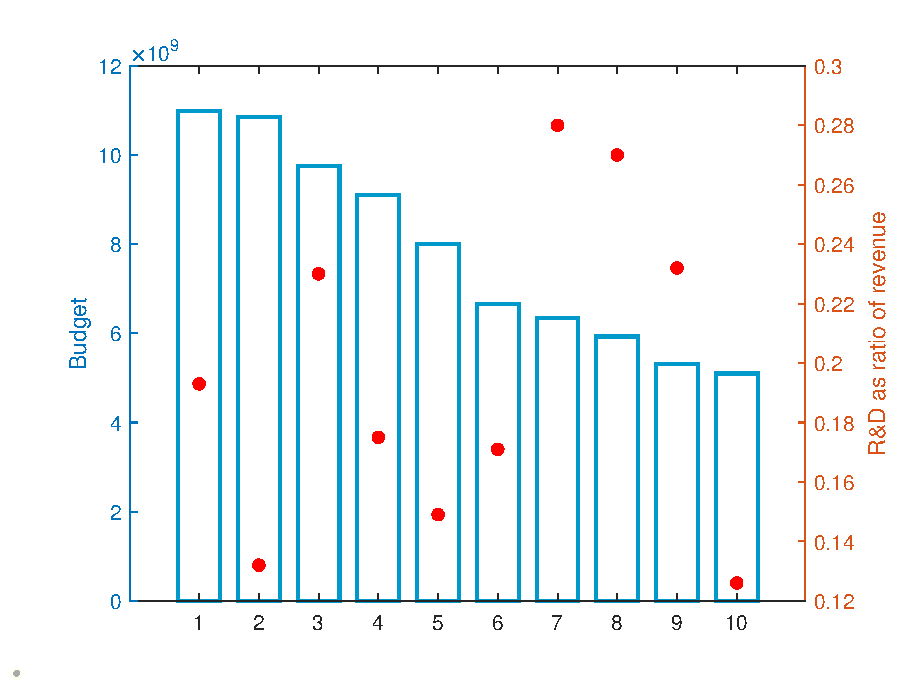
\includegraphics[width=1\linewidth]{fig1}
	\caption{2018年全球前十制药公司研发投入及比例}
	\label{fig:fig1}
\end{figure}
,而国内仅有恒瑞医药在2018年投入比例达到15.3\%,其余几乎都在10\%以下。且国内企业研发投入偏低,如恒瑞医药2018年研发投入为26.70亿元,即使与全球前十中最低的50亿美元相比,也存在较大差距。如图\ref{fig:fig2}所示:除了研发投入,国内提出上市申请的创新化学药与生物药都有着上升趋势,最近几年有明显增长\citep{RN19};
\begin{figure}[tb]
	\centering
	\subfigure[2008至2018年国内申请上市创新药]{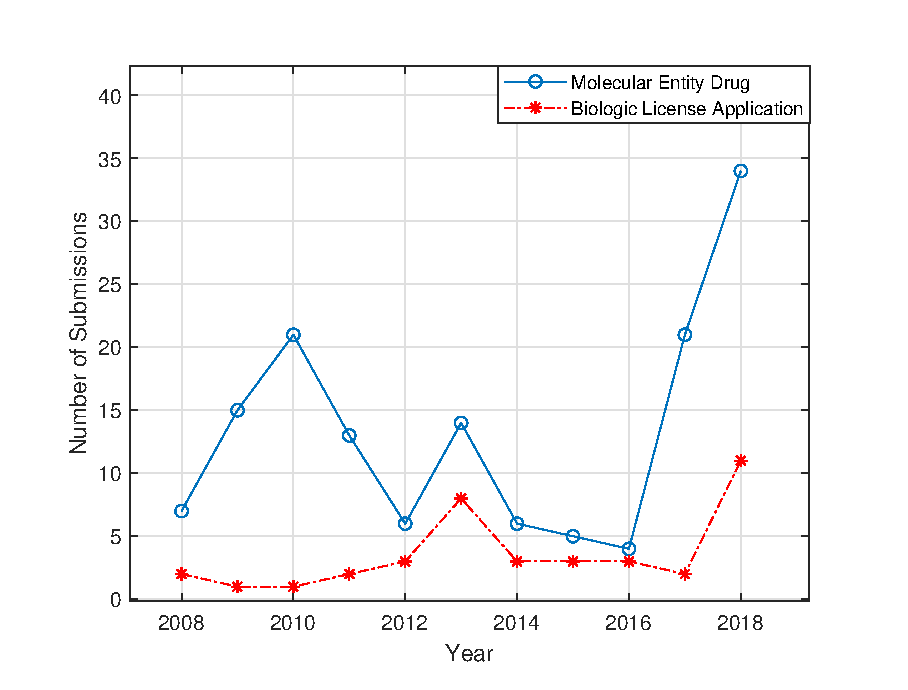
\includegraphics[width=1\linewidth]{fig2-2deng}}
	\\
	\subfigure[2008至2018年国内批准上市创新药]{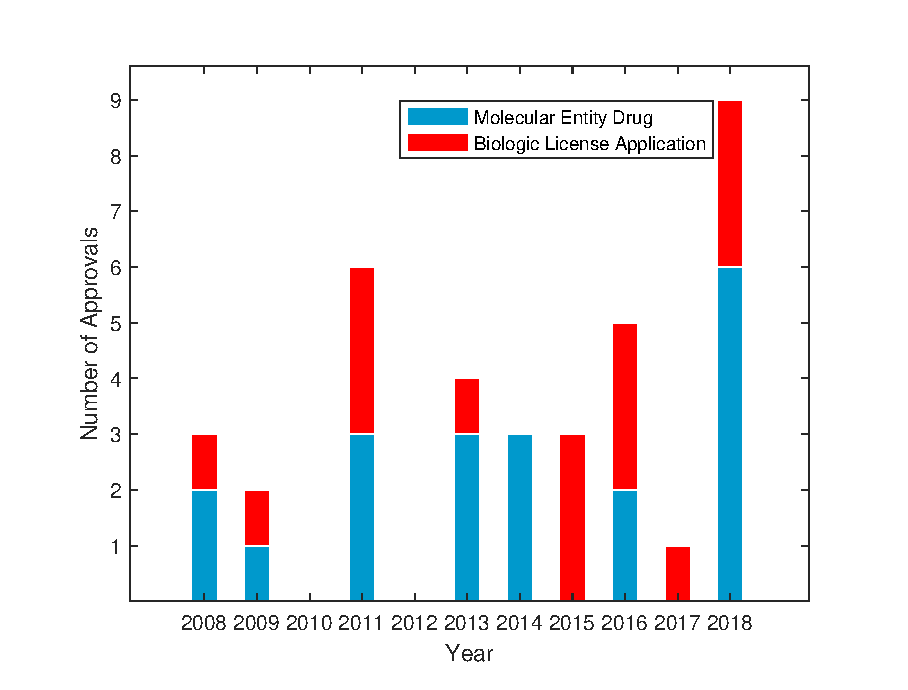
\includegraphics[width=1\linewidth]{fig3-2deng}}
	\caption{2008至2018年国内申请上市以及批准上市创新药物}
	\label{fig:fig2}
\end{figure}
而过去审核流程长,成功上市的创新药较少,甚至存在没有新药上市的年份,不过随着审核时间的缩短,上市的创新药数量已经存在上升趋势,未来也会更加明显。

\chapter{企业介绍}

		\section{北京福元药业有限责任公司}
		
		北京福元药业有限责任公司于1999年成立,前身是1956年成立的北京生化制药厂,其原名为北京万生药业,近期更名为北京福元药业。该公司为新和成控股集团旗下的子公司,专业从事药品、医疗器械研发、生产和营销的高新技术企业。近期公司更名为北京福元药业。福元药业是专业从事药品、医疗器械研发、生产和营销的高新技术企业,目前主要进行化学药的仿制及生产。
		
		福元药业总部及研发生产基地位于北京市通州区工业开发区,同时在沧州有高端原料药生产基地\citep{RN31}。企业主要分为研发、生产、营销和职能四个系统,其中生产和研发系统又下分为药物、器械生产研发的两个方向。药物研发部门由研发总监下辖医学部、合成部、药学部、注册部、项目管理部,药学部分为分析组和制剂组\citep{RN33}。
		
		福元药业在通州的研发中心现有员工130余人,硕士占比为60\%以上,博士6人,其余为本科生或大专学生。其研发中心拥有5000余平米的现代化实验设施和场所,具备原料药、片剂、胶囊剂、颗粒剂、注射剂、缓控释制剂、纳微化制剂等多种国内先进技术水平的原料及制剂的开发能力,并曾与北京化工大学、中国医学科学院医药生物技术研究所、沈阳药科大学、上海应用技术学院等科研机构开展合作,如曾与北京化工大学共建了被认定为“北京市纳微化结构药物工程技术研究中心”的万生-北化纳微化结构药物联合实验室。该实验室希望通过不同的制粒技术,制备出纳米化的药物,并投入生产应用。福元药业倡导“老师文化”,鼓励学习和模仿,自身研发也集中于化学制药领域,并始终专注于仿制多发性疾病的临床急需品种,建有符合GLP(Good Laboratory Practice,药物非临床研究质量管理规范)标准的新药研发中心\citep{RN30}。
		
		福元药业已完成18个品种的上市研究,现已拥有国家药品生产批件的制剂和原料药共计49个品种,其中包括“复方$\alpha$-酮酸片”、“奥美沙坦酯片”、“盐酸莫西沙星片”、“曲美他嗪片”、“氯沙坦钾胶囊”、“文拉法辛缓释胶囊”、“匹维溴铵片”等7个国内首仿制剂品种,申请专利54项。目前在研品种50余个,且30余个品种已获临床批件\citep{RN32}。
		
		可以检索到的福元药业的专利大部分为药物制剂的专利,如“药物瑞格列奈药物制剂的制备方法”、少部分物质合成专利,如“制备罗氟司特中间体的方法”,以及物质检测专利和早些时候的包装盒专利。客观来看,其拥有的高价值专利较少,且今年来发出的专利书目与以前相比有减少的趋势。
		
		\section{江苏先声药业有限公司}
		
		江苏先声药业有限公司成立于1995年,是中国领先的研发驱动型制药企业,曾是中国第一家登陆纽约证券交易所的生物和化学制药公司。先声药业总部位于江苏省南京市玄武大道699-18号,在南京、上海有两家研发中心,且正在筹备建立波士顿创新中心;也有南京先声东元药业(最大生产中心)、先声中人制药(新剂型生产)、海南先声药业(出口产品生产)、山东先声生物(大分子药物生产)四家进行药物生产的子公司;以及江苏先声药业、上海先声药业两家负责营销的子公司。同时先声在伦敦和香港也设有分公司。先声药业现也在新泽西建立了办公室,寻求合作机会;先声药业也曾与清华大学胡跃飞老师有合作实验室。现产品研发方面,仿制药与创新药的资源、人力投入比例约为1:1,未来将有更多的资源向创新药方向倾斜\citep{RN34}。
		
		另外,先声药业与跨国药企和生物技术公司(包括BMS、药明康德等制药企业)开展了多种形式的国际合作,并于2013年开创了百家汇创新平台模式。百家汇是开放的创新创业平台,先声对于有创新意愿的小公司进行投资,创新成功后小公司可以选择依附于先声或者脱离。百家汇创新平台自创立以来已累计汇聚逾百个科技创业公司和项目团队。先声药业还投资了其他领域公司,且获得了较大成功,其中Oxford Nanopore和Verltns Genetics曾被《麻省理工科技评论》全球最聪明的50家公司。
		
		先声药业的企业宗旨是“Making Better Medicines Available to Patients Sooner”,即“让患者早日用上更好药物”,企业的核心价值观是“诚信、杰出、奋斗、主动作为、客户第一”。在这些理念的引领下,先声药业自2000年开始进行新药的自主研发,长期以来研发投入超过10\%,主要围绕临床上多发病、常见病以及恶性肿瘤研发药物,目前已经成功研发并且上市的有恩度(抗肿瘤药物)、中人氟安(长效的抗肿瘤制剂)、艾得辛(类风湿关节炎药物)为代表的全球首发创新药,也有再林(抗感染药物)、必存(脑神经保护剂)、安信(全合成的超级抗生素)等全国首发的创新药。除恩度是比较成功的生物制药案外,先声的产品结构还是以化学制药为主\citep{RN35}。先声药业的相关成果曾获国家科技进步二等奖、国家技术发明二等奖等。先声药业还是全球8个个基金的LP(Limited Partner,有限合伙人),基金资金总规模超过30亿美元,先声也出资了2.1亿美元,将许多生命科学领域前沿成果引入中国。
		
		
		先声药业可以检索到的专利信息有200余条,基本都为发明专利,涉及物质的制备、检测、应用等多个领域。先声药业也因相关成果获国家科技进步二等奖、国家技术发明二等奖,并承担了20项国家重大科技专项。
	
		\section{上海合全药业股份有限公司}
	上海合全药业股份有限责任公司是药明康德集团旗下的一家子公司,2003年从药明康德工艺研发部门独立出来。合全药业拥有化学创新药物研发和生产能力,主要从事小分子药物生产、药用化合物研发和药物生产放大、制剂方向的工作,是全球CDMO领域的领军企业,并致力于为全球合作伙伴提供从API(Active Pharmaceutical Ingredient,原料药)到制剂,高效、灵活、高质量的一站式解决方案。
	
	合全药业的原料药研发、制剂研发基地位于上海市外高桥保税区,在上海金山及江苏常州设有原料药生产基地;在江苏无锡有进行制剂商业化生产的公司;同时在美国圣地亚哥也有进行原料药研发与生产及制剂开发的公司\citep{RN37}。
		
		合全药业的公司部门包括工艺研发与商业部、制剂部、工艺分析及质量控制部、质量保证部、API生产部以及商务运营部,拥有一支由千余名经验丰富的研究人员和科学家组成的大规模化学工艺团队\citep{RN36}。
		
		合全药业的理念是“诚实敬业,共苦共享,做对的事,把事做好”,并希望“让天下没有难做的药,难治的病”,在此指导下,合全药业专注于CDMO服务,为客户提供合成路线筛选、工艺开发,优化和放大、确定起始原料,中间体和API的质量控制策略、工艺验证等服务,目前国内约10\%的已上市药物是由合全药业研发而成。合全还拥有能在cGMP(Current Good Manufacture Practices,动态药品生产管理规范)标准下生产公斤级到吨级的中间体和创新原料药的生产设备,其中上海金山工厂已通过全球8个监管机构的批准,包括美国FDA、中国NMPA、欧盟EMA、澳大利亚TGA、加拿大卫生部、日本厚生劳动省、瑞士药检局、新西兰MPI。
		
		可以检索到的上海合全药业股份有限公司的专利共78条,专利内容以药物全合成路线为主。其中上海合全药业股份有限公司为第一作者的专利有13条,包括发明授权3条;13条专利中10条与全合成路线有关;常州合全药业有限公司拥有15条专利,其中8条与化学合成有关;上海合全药物研发有限公司共拥有54条专利,其中有35条与化学合成路线有关;上海合全医药有限公司拥有10条专利,以制剂技术方向的专利为主。
		
	\chapter{调研成果}
	支队调研主题确定为制药企业创新能力,但考虑到“创新能力”概念较为模糊,其影响因素多,并结合前期调研时了解到的制药企业的一些特点,本文将其细化为企业的研发模式,合作关系,以及实验设施,员工待遇等其他方面。同时通过对国家相关政策,及调研时企业高管与研究人员的回答,来了解支队所调研企业的创新能力及前景。
		\section{药物研发}
	医药行业的药物研发可以简单地分为仿制和创新两种,仿制药通常指对过了专利保护期的原研药进行改进,而创新药则是自主研发出新的活性成分。在国内提倡创新的大环境下,创新药的研发逐渐得到重视。在此部分中,将结合国内研发现状,对企业目前所采取的研发模式及未来的研发偏向进行分析。
				
			\subsection{仿制药}
			我国总体仿制药市场规模达到5000亿元左右,约占总药品消费市场的40\%,但产业集中度极低,国内CR8(Concentration Ratio  8,规模最大的前八家企业的产业集中度)占比仅达到19.92\%,与印度的52.31\%、美国的52.96\%相比差距明显。根据2017年的数据,在国内3244个化学药物品种中,262个品种占据了注册文号总量的70\%,可以较明显地看出国内仿制的低水平及其所导致的恶性竞争,这也导致大多数企业追求药物数量而非质量,从而导致仿制药与原研药在药效上差距大,行业整理盈利少,平均毛利润仅达到5-10\%,远低于国际的50\%左右\citep{RN21}。但随着最近仿制药一致性评价的强制推行,该现象得到缓解。
			
			仿制药从研发到申报需要一至两年的时间,大致要经过调研立项,优化并确定合成工艺、工艺放大、稳定性及质量检测等步骤\citep{RN22}。优化及确认工艺又可细分为合成API、配置辅料、制粒、包衣等。其中前两个步骤是进行工艺优化的核心,企业可以通过改进合成路线降低成本,也可以改变原研药辅料组成或配比,较大幅度地提高药效或减轻副作用,这也是国内仿制药由以前“me worse”或“me too”走向“me better”的关键步骤\citep{RN12}。
			
			过去几年中,国内仿制药主要在获得审核批文的时间及产品的价格上竞争,导致许多研发能力不强的公司得到发展,如今研发成本升高到千万级别,大部分质量较差的药无法让企业获益;并且国家对仿制药质量的要求也变高,强制推行了药物一致性评价,并加速审批流程以让优质药物早日上市,这使得一批小企业被淘汰。与以往盲目选取仿制目标不同,如今的仿制企业大多在经过了对自身研发能力的定位,对生产、销售线匹配程度的调研,以及对市场需求的评估后,再选择进行仿制的原研药。之后企业大多采取争做国内首家仿制药的策略,即在专利期内研发出更好的仿制药,在原研药专利期过期后立刻申请上市销售,进行发展。在仿制过程中,由于存在对原研药关键数据或关键结构的保护,如何高效,高质量地完成研发便是真正考验企业研发团队的地方。
			
			福元药业共有两个合成原料药小组,每个组同时进行二至三个项目的研发,并配有专门的分析部门,主要分析原研药中API含量及杂质含量;药物合成后,转至制剂组,尝试对辅料进行改进;之后再进行放大,最后投入生产。福元的基础实验设施较为完备,但某些相对昂贵的仪器往往只有一台或几台,如其气相色谱仪便存在不够使用的情况。福元每年大约会进行30种药物的研发,并有十种左右申请审核,可以看出其研发速度较高,如其仿制的列净类药物达格列净,用了一年时间改进合成工艺并成功合成API,再经过半年完成制剂及放大,目前正在申请审核。尽管福元药业申请的仿制药数量较多,但上市后的药物只有不到40\%能得到预期的收益,实际效果并不太好。
			
			福元药业是国内小型制药企业的一个较典型的例子,它们往往只进行仿制,并仍然希望以药物数量弥补质量上的不足;而先声便是较为成功的中大型企业的典型,其完成的仿制药,如必存、安信、再林等六种药物都成功成为国内首家上市,并且这类企业对药物的仿制更多地是为创新药研发提供足够资金。
			
			
			\subsection{自主研发}
			我国自主研发起步较晚,因此统计至2017年,在我国现有的18.9万个药品批文中,约95\%是仿制药批文\citep{RN21}。并且由于新药研发周期长,国内上市的新药数量与国外相比差距较大。美国约占据了一半以上的全球上市新药,而中国仅有2\%左右\citep{RN23}。但国内新药研发的前景越来越好,进行创新药研发的企业受到了更多的支持,在创新药研发上也取得了一定的突破,逐渐打破了国外制药企业的垄断:如恒瑞医药的甲磺酸阿帕替尼的上市,打破了国际上小分子靶向治疗新药的垄断;康弘药业的康柏西普(治疗眼底黄斑变性)和西达苯胺(治疗外周 T 细胞淋巴瘤)的上市打破了国际生物药垄断\citep{RN24}。
			
			创新药研发周期远远长于仿制药,通常需要十到十五年,最近有些药物能缩短到十年以内,但整体耗时较长。新药研发首先需要找到靶点与先导物,但考虑到寻找新的靶点所需工作量大,制药企业大多都从已知靶点出发,寻找新的先导物,之后便会经历先导物优化、临床前研发、临床研究等阶段,其中临床前研发又能继续细分,以提高药效如图\ref{fig:flow1}所示。由于国内企业仍存在资金、技术等多方面限制,大多数进行创新药研发的企业,也会研发仿制药,以来带资金流动;仅有一些小企业会采取完全自主研发的方式,并希望通过成功研发得到进一步发展。
			
			\begin{figure}
				\centering
				\includegraphics[width=0.3\linewidth]{flow1}
				\caption{新药研发全流程图}
				\label{fig:flow1}
			\end{figure}
			
			福元药业考虑到自身研发团队组成及创新药前期研发耗时长的问题,没有进行自主研发的计划;而先声药业已经成功从仿制药研发转型成了仿制与创新兼并的企业,目前在仿制药与创新药上资源分配(人员及资金)大致为1:1,在研发上投入比例也接近10\%,并逐年提高。至今先声药业已成功研制出了恩度、中人氟安、艾拉莫德三种全球独家创新药,还有依达拉库右旋茨醇(复方试剂)、布拉克索斯(治疗帕金森病)等多种产品正在审核中。先声也因为自身在创新药上的成果,被批准成立全国12个重点实验室之一的转化医学与创新药物国家重点实验室。近年来,生物制药逐渐兴起,先声也进行了生物新药的研发,并通过与国外企业合作提高自身研发技术与能力,在该领域有了较好成果,如成功合作研发出的单抗类药物奥玛思普。除此之外,先声还主动向精准医疗领域上发展,这拓宽了自主研发的范围,从单纯的制药扩展诊断,给了其他企业发展的机遇。
			
			\begin{framed}
				未来仿制药竞争将集中在药物质量上,同时由于首仿药能够占据更多市场份额,只有研制高难度的仿制药,并成功抢到首仿,才能较长时期维持高盈利状况。而对于类似于福元药业的纯仿制企业来说,需要有持续开发新产品的能力以适应产品盈利周期缩短的现象,因此,这类企业未来发展将会受到极大限制。并且随着“4+7带量采购”的实行,药品质量标准提高,价格下降,对企业在生产质量,成本上提出了更高要求。这使得该类企业的经营必将更加困难,尽管仿制药本身对于我国仍然有重大意义,但单纯通过仿制药数量,甚至通过仿制药质量带来足够收益的研发模式已经不再适合,此时企业应该主动转型,调整企业自身定位及研发团队分配,着手创新药物研发。转型期间也可以通过与其他企业或研究所间的合作,促进这一过程,得到进一步的发展。
			\end{framed}
			
		\section{合作}
		合作是制药企业常常采取的一种策略,企业可以通过合作组成新的创新主体,在保持核心机密的同时共享其他信息,从而提高自身创新能力。合作通常可以被分为与高校和研究所,或与其他企业的合作。在此部分中,将分析企业对于合作的态度、合作的方式,以及合作的成果。
		
			\subsection{与高校或研究所}
			在与高校或者研究所的合作过程中,由于长期经验的积累,形成了以产学研相结合为主的合作形式。作为公司技术人员的来源,产学研这条道路输送着新鲜的血液,同时也不断将实验室中的知识转化为工厂的实际成果。但就支队所调研的企业而言,产学研与大众的认知相比存在较大的偏差,产学研结合的规模及目前对企业的益处都相对较小。
			
			不可否认的是,通过与高校或研究所的合作,企业可以充分接触到新的研究开发新药的思路,推动企业在研发上的突破;但由于企业对于实际应用的要求更高,而高校或研究所更注重基础研究,这种类型的合作往往难以实现,即药物研发和生产两端的差异,会较大地影响到企业对与高校或研究所合作的态度及方式。如福元药业与高校的合作极少,且主要集中在思想理念与技术引导上,而在涉及到相关的生产方面,依然由企业负责。
			
			为了推动国内产学研结合,国家开放了相关政策,使得某些拥有好的想法却缺少资金的高校教授或者科研人员能直接与企业合作对接,实现项目的产业化。当企业寻找到有意义的合作项目时,后期成果分配便通过双方贡献确定,如当高校的工作具有极强的创新性,则专利权属于高校,并通过专利许可(优先授权)的方式形成共享。
			
			先声药业便通过类似模式进行合作:高校实验室提供思路,公司在引入相关思路并进行合理评估后,决定是否使用或拓展;同时,作为一家具有良好战略眼光的企业,先声在拥有全球8个基金LP的基础上,紧跟科技最新成果,聚焦哈佛、牛津以及其他高校,把握前沿,展开相关项目的合作。相比于先声药业的源头创新来说,合全药业的创新更集中在实际生产环节,针对于这样的需求,合全药业与高校的合作显得不太密切。就目前合全药业与高校的合作情况来看,合作的回报低于投入,企业更希望通过此吸引优秀的学生前来入职,而非直接创造收益。
			
			
			\subsection{与企业合作}
			
			相较于与高校或者研究所之间的合作,企业间合作就更加注重于知识,技术及相关理念的双向传递与交流。在同样的社会背景之下,企业之间通过合作,转换知识、信息与资源,可以帮助企业更好地把握当下的需求与未来的方向,以迅速实现相关技术的更新,提高公司整体的创新实力。而在这个合作过程中,为了保证有充足的竞争力,企业间的合作表现出相对封闭的状态,会对于核心的信息予以部分甚至全部的保留。
			
			福元药业并未与其他企业进行合作,这在当今的产业链逐步成熟、分工愈发明确的大背景下,呈现出一定的滞涩性。而对于这个现象,所展现的更多的应当是现今的小型医制药企业业在市场上面临的困境——举步维艰且只能够在自我旧模式“坚守”,这也是一种无奈的选择。
			
			在小型企业面临此状况时,先声药业为他们指出了一种方向。依据自身的实力与地位,先声创设了一个开放式的创新社区——百家汇。百家汇是一种类似于孵化器的合作模式,有着众多小型制药企业参与其中。拥有创新技术的小型企业得到先声的投资,而企业成功完成创新后,先声也能获得一定利益。除此之外,先声还有多种与其他企业的合作方式:关注一些小型企业的早期项目,并在完成评估之后通过专利或技术转让、买入公司等方式进行吸收;与纯外包公司进行合作,更有针对性地发展自己的新药开发创新实力;由其他公司提供技术,先声向其投资,最后成功共享,这也是先声采取得最多的一种模式。在国际上,先声药业选择“走出去”发展战略,与多家大型跨国制药公司进行合作,并开展全球创新投资,获得相应的开发权,如先声投资了Merus在双抗药物上的研发、Roche在精准医疗上的研发。通过这样的举措,先声实现了与国际接轨,扩展了在全球视野下的创新发展思路。此外,值得一提的是,先声药业还投资了其他领域的公司,且取得了多点开花的良好成效,如在2017年,其投资的两家公司入选《麻省理工科技评论》“全球最聪明的50家公司”,从某种意义上来讲,这也更多元化地促进了先声实力的增强,为实现创新注入了新的不一样的活力\citep{RN5}。
			
			相较于福元与先声药业,合全药业业务完全集中在CDMO上。除此之外,合全药业也通过与其他企业开展学术会议等形式,推动公司进步。
			
			
			
			\subsection{CMO/CDMO}
			为了降低研发成本,提高企业资产的运营效率,一些企业将部分研发工作交给了更专业的团队,由此兴起了CRO以及CMO/CDMO服务。其中CRO主要提供新药开发服务;CMO则提供药物生产时工艺开发及后续服务;CDMO与CMO相比则更强调对工艺的优化,是在CMO上的进一步发展。如今跨国大公司希望将更多资金与人员投入到新药发现及市场营销上,因此与药物生产更相关的CDMO服务正快速发展,所占市场规模也逐年提高,如图\ref{fig:fig4}所示\citep{RN25}。
			
			\begin{figure}
				\centering
				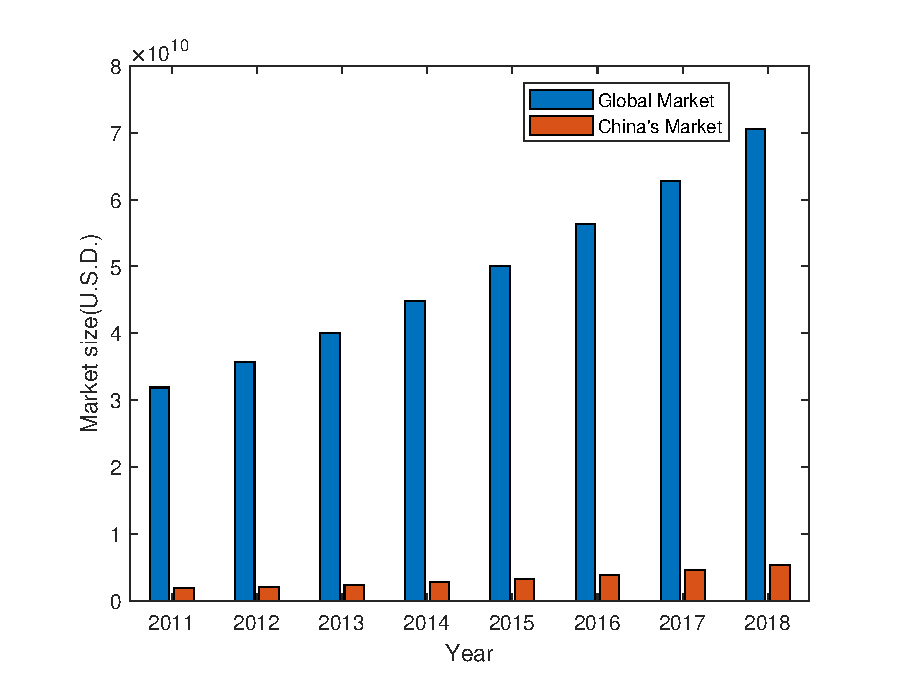
\includegraphics[width=1.0\linewidth]{fig4}
				\caption{2011-2018年全球及中国CMO/CDMO行业规模}
				\label{fig:fig4}
			\end{figure}
			
			通常来说,CRO作为制药企业的一种可借用的外部资源,可在短时间内迅速组织起一个具有高度专业化和丰富临床研究经验的临床研究队伍,降低整个制药企业的管理费用\citep{RN10}。CDMO则是为企业提供从研发到生产一体化的服务,与CRO相比更能方便企业对产品进行管理,提供相关服务的企业也会在过程中保证每个阶段的质量,让企业能专注于后期的市场营销。无论是CRO还是CDMO,都分为客户提供订单及给客户分配实验人员两种模式,如CRO中的FFS(Free-For-Service),FTE(Full-Time Equivalent)。其中FFS主要是客户提供定金,企业在一定时间内完成研发项目,收益与风险较高;而FTE则是企业将一个研发团队租给客户,客户支付人力成本,收益与风险均较低。
			
			在这种新的模式出现的背景下,作为小型企业的福元药业考虑到公司本身的实力、研发团队的方向以及市场评估等多方面因素影响,选择了不将研发项目外包,根据团队的特性继续发展。而对于先声药业这种具备一定实力的企业来说,他们选择了积极参与CDMO新潮之中。先声以自己的新药发现能力为依托,通过参与CDMO,进一步提高公司的生产效率,同时也能够更加专注地将自己的研发团队集中在新药的研发上,进行药物源头的创新。CDMO作为一种需要两端参与的药物开发生产模式,在承接项目一端,同样也需要投入,这也是合全药业进行的研发工作。对于类似于合全的进行CDMO服务的企业,一般来说,是由BD(Business Development)在完成对项目的审核评估并决定接受之后,交给研发团队进行研究开发。
			
			在长期从事CDMO的过程中,合全已经积累了相当多的经验,具有雄厚的实力。每年,合全药业会承接近1000个项目,基本能够全部完成,并且在目前中国已经上市的药物中,约10\%都有着合全药业的参与。这一切,也都离不开合全药业在逐步探索承接外包模式时对于自我研发的不断提高。合全药业CDMO服务的根本在于预见生产中可能出现的问题并予以解决,同时其公司内部的研发团队都秉持着“No Talking No Sharing”的原则,以防止客户的需求及目标,每个团队之间保持着相应的独立性。在另一方面,合全药业始终未从事自主创新,这同样也是战略选择:通过这样的方式,让专业的人做专业的事,实现做到极致、不分心的目标,以使客户利益最大化,达到双赢;其次,这样的选择以使得公司不会轻易受到能力、技术、产能的限制,也可以使客户更加放心地与合全合作,不必担心药物源头被利用,使得公司在行业之中拥有了稳定的立足点与长远的发展空间\citep{RN3}。
			
			
			\begin{framed}
				在追求创新的大背景下,整个产业链更加规整化,分工更为细致而明确,与之相伴而来的,便是对创新的要求变得更加显著且阶段化:既可以在新药开发上面提出新的思路,也可以在后续的研发上实现新的突破,但不可避免地,也可能因为一时失误使得企业陷入困境,此时寻求适合企业进行合作的方式是一种较好的解决办法,但福元药业对合作的拒斥让自身陷入僵局,而先声与合全都找到了最佳的合作方案及合作中的位置,使得企业能将资源更合理,集中地分配到更具体的方面,以提高企业自身创新能力。
			\end{framed}
			
			\section{政策}
			除了企业自身采取的策略外,国家相关政策对于企业发展也有较大影响,政策的偏向能一定程度上决定企业的研发偏向,从而间接影响企业创新能力。在此部分中,将结合相关理论对调研得到的内容进行分析。
			\subsection{理论分析}
			\subsubsection{宏观政策}
			
			根据经济学原理,企业的研发等活动具有正外部性,因为其他企业或个人可以利用研发活动所得的成果获取收益,而这部分收益并未被计算在企业收益内。这种市场环境下的供求曲线如下图所示,表中的“需求”曲线对应的价值是企业的研发活动给企业带来的收益,“社会价值”曲线对应企业的研发活动给企业和其他人带来的收益。研发活动的社会最优量大于研发活动的均衡量(横坐标轴)\citep{RN29}。
			%N.格里高利·曼昆 《经济学原理》第7版,第215页,第218至220页,北京大学出版社
			\begin{figure}[ht]
				\centering
				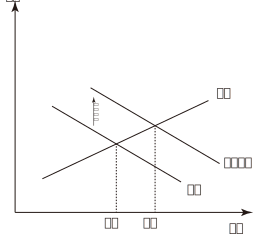
\includegraphics[width=7cm]{fig5.png} %供求曲线图
				\caption{正外部性条件下的供求曲线图}
				\label{fig:fig5}
			\end{figure}
			
			要使研发活动的均衡数量等于社会最优量,市场管理者可以通过一些手段鼓励企业进行研发,如通过税收等补贴手段降低企业生产的成本,在这种情况下研发的供给曲线向下移动,均衡数量增加至原有的最优数量\citep{RN14}。
			
			\begin{figure}[ht]
				\centering
				\includegraphics[width=7cm]{fig6.png} %供求曲线图
				\caption{补贴对市场的影响}
				\label{fig:fig6}
			\end{figure}
			
			在政策的实际应用中,很难具体确定出市场的供求关系,因此供求关系只能定性地明确市场管理者需要对研发活动进行补贴,而很难具体确定补贴的数值\citep{RN13}。
			
			\subsubsection{企业的生产成本}
			
			如前所述,企业的生产成本分为固定成本和可变成本。固定成本只需要进行一次投资,而可变成本随着企业的生产活动需要不断进行投资。在一段时间内,企业的平均成本是总成本和产量的比值。一般情况下,企业的生产遵循边际成本递增原理,即当企业的生产量越高,企业每多生产一单位产品的成本越高。
			
			\begin{figure}[ht]
				\centering
				\includegraphics[width=7cm]{fig7.png} %供求曲线图
				\caption{企业的生产成本}
				\label{fig:fig7}
			\end{figure}
			
			在制药企业的生产经营中,仪器和设备属于固定成本,而人员薪资属于可变成本。随着产量的增加,平均固定成本呈现一个下降的趋势,而平均可变成本呈现一个上升的趋势。当企业的生产达到一定规模时,平均可变成本势必超过平均固定成本,进而成为成本中最主要的部分。因此在制药企业中,预期的主要研发支出是人员薪酬方面的支出。
			
			\subsubsection{企业的决策}
			
			在市场环境下存在着不同规模的企业,有些企业的规模较大,生产、研发能力较强,另外一些企业的规模则相对较小。在同一环境下,这些企业可能会采取不同的决策,决定是进行创新还是进行仿制。
			
			考虑一个由两家制药企业组成的市场,企业A的规模较小,企业B的规模较大。A、B两企业都可以选择进行研发还是进行仿制。对于任意企业,选择研发时需要投入3单位的成本。若企业A选择进行研发,则A可获得10单位的收益,若企业B选择进行研发,B可获得15单位的收益。选择仿制的企业比选择研发的企业收益少5单位,特别地,如果两个企业同时选择进行仿制,就没有收益。据此,列出A、B两家企业的收益,如表1所示:
			
			%胡运权 《运筹学教程》第4版 清华大学出版社(不过我没带书回来)
			
			\begin{table}
				\centering
				\begin{tabular}{|c|c|c|}
					\hline
					\quad  & A:研发   & A:仿制    \\
					\hline
					B:研发 & A:7;B:12 & A:10;B:12 \\
					\hline
					B:仿制 & A:7;B:5  & A:0;B:0   \\
					\hline
				\end{tabular}
				\caption{A、B两家企业的收益}
				\label{tab:tab2}
			\end{table}
			
			根据A、B企业各自的收益可以得出当前市场条件下的Nash均衡策略:规模相对小的A企业倾向于选择仿制,B企业倾向于研发,此时企业A的收益为10,企业B的收益为12。将这个结论拓展的实际市场中,可以得出小企业通常会选择仿制,而规模更大的企业的研发比重会更大的结论。但由于模型的限制,以及制药行业成本高昂和技术不平衡的行业现状,即使是国内规模较大的制药企业也难以完全负担全部成本以进行完全独立的药物研发。
			
			\subsection{宏观政策}
			
			药物生产行业是创新驱动型产业。但药物的研发需要投入大量成本,这些成本包括仪器设备、场地等固定成本和人员薪酬等可变成本。研发成本高促使企业倾向于进行药物的仿制和改良,而不是从头进行药物研发、生产、临床测试等研究活动。为激励企业进行创新,世界各国从宏观层面对研发活动进行支持,如提供税收优惠等。这一系列支持政策主要从降低企业研发的成本或提高企业收入入手。
			
			在对不同制药企业的调研过程中我们了解到宏观政策能对企业的决策产生重大的影响,通过查阅相关的文献资料,我们了解到制药行业的监管与与政策整体分为经济型规制与社会型规制\citep{RN26}。经济型规制主要涉及到企业在市场上的行为,主要分为价格管制、集中采购规制、市场准入规制。
			
			
			\begin{enumerate}
				\item 市场准入规制规定了企业进入药物市场所必须具备的资质条件,提高了进入市场的门槛,有利于规范整个市场的生产经营活动。2016年山东的非法疫苗事件表明医药市场的正常运作需要完善的法律支持,进入市场的企业也应具有完备的资质。
				
				\item 价格管制限制企业出售药品的最高价格。一般认为,设置限制性价格上限会降低企业的生产激励,导致供给不足的情况。但根据我们的调研结果,部分企业会对药物制定一个较高的价格。由于药品是生活必需品,其需求弹性相对较弱,在价格有大幅度提高时药品的需求量并不会有明显的下降。相关文献表明,对高价药实施适当的价格管制措施可以激励其他企业的创新活动\citep{RN28}。然而,通常情况下仿制药相对于创新药的价格较低,企业生产仿制药的利润更少。此时对药品设置的价格管制政策更可能导致制药企业停止进行生产,转而生产利润更多的药物。有研究认为,价格管制会对企业的创新产生反向的激励\citep{RN27}。
				
				\item 医疗保险制度对需求方加以补贴,相同药品价格下药品需求量增加,为制药企业的创新活动产生正向的激励。但医疗保险的资金来源依然是政府税收,药价过高时会对政府产生较大压力。
				
				\item 社会型规制侧重企业的药物产品对社会的影响,如药物不良反应规制。
			\end{enumerate}
			
			由于创新药和仿制药在成本和收益方面的不同,国家采取了不同的政策扶持制药企业的发展。
			
			\subsection{创新药的支持政策}
			
			目前我国在创新药方面落后于美国。癌症等疾病的药品依然由外国企业垄断,当对这些药物实行价格管制时,这些企业可以选择退出中国市场使得价格管制措施不能收到预期的效果。因此需要通过其他手段打破外国企业在创新药方面的垄断,对国产创新药进行支持\citep{RN11}。
			
			2018年7月,药监局发布《关于调整药物临床试验审评审批程序的公告》,开始实行临床试验申请到期默认制。中国制药企业在提出临床试验申请后,若国家药品监督管理局在一段时间内没有提出异议,企业可以自行进行临床试验环节的研发。这一政策同时缩短了制药企业的研发时间和研发周期,缩短了临床试验的审批流程。
			
			另外,国家药品监督管理局优先审批与进口创新药拥有相同适应症的国产创新药以及生物仿制药,%这一点我也找不到具体来源……原文在知乎上……https://www.zhihu.com/question/20212827
			在一定程度上动摇了外资企业的垄断基础,同时对国内制药企业的创新活动产生正向的激励。
			
			2019年发布的《深化医药卫生体制改革2019年重点工作任务》中已经将药品集中采购和使用为突破口进行医疗改革提上了日程。这一政策在一定程度上分担了消费者的经济压力,有利于提高创新药品的销售量,提高了企业的收入因而激励企业进行创新。
			
			\subsection{仿制药的支持政策}
			
			2000年至2015年间, 出现了恩度等一些创新药,但我国自主知识产权的创新药的比例不高,仿制药的质量参差不齐且产能大量过剩,因此,经过讨论,我们认为,国家在仿制药方面采取的主要措施应是:
			
			\begin{enumerate}
				\item 加强仿制药市场的监管,完善市场准入条件;
				\item 整治、淘汰落后产能;
				\item 鼓励企业仿制需求量大或针对危重疾病的药品;
				\item 鼓励仿制药企业转型升级,逐步进行自主研发。
			\end{enumerate}
			
			国务院2018年发布的《国务院办公厅关于改革完善仿制药供应保障及使用政策的意见》中提及了“促进仿制药研发”。其中明确表明:要制定鼓励仿制的药品目录,并加强仿制药品的技术攻关以降低成本或对原技术方案进行改良。
			
			\begin{quotation}
				\itshape
				……以需求为导向,鼓励仿制临床必需、疗效确切、供应短缺的药品,鼓励仿制重大传染病防治和罕见病治疗所需药品、处置突发公共卫生事件所需药品、儿童使用药品以及专利到期前一年尚没有提出注册申请的药品。
			\end{quotation}
			
			截至2019年7月,国务院已经发布《第一批鼓励药品仿制目录建议清单》,其中包含了针对艾滋病、白血病等严重威胁人们生命健康的疾病的药品。除了提出建议仿制药品目录以外,我国还在进一步加强对药品质量的监管,推进仿制药质量和疗效的一致性评价。这一政策从药品的治疗效果入手规范仿制药市场,逐步淘汰无法得到预期疗效的仿制药品,进一步规范了仿制药企业的生产行为。
			
			\begin{quotation}
				\itshape
				对2007年修订的《药品注册管理办法》施行前批准的仿制药,分期分批与被仿制药进行质量一致性评价,其中纳入国家基本药物目录、临床常用的仿制药在2015年前完成,未通过质量一致性评价的不予再注册,注销其药品批准证明文件。药品生产企业必须按《药品注册管理办法》要求,将其生产的仿制药与被仿制药进行全面对比研究,作为申报再注册的依据。——《国家药品安全“十二五”规划》,2012年1月20日
				
				对通过一致性评价的药品品种,按程序优先纳入基本药物目录。对已纳入基本药物目录的仿制药,鼓励企业开展一致性评价,未通过一致性评价的基本药物品种,逐步调出目录。鼓励医疗机构优先采购和使用通过一致性评价、价格适宜的基本药物。——《国务院办公厅关于完善国家基本药物制度的意见》,2018年9月13日
			\end{quotation}
			\section{其他}
			对企业创新能力的衡量比较复杂,支队在调研中也了解了关于三家企业的其他情况,如员工组成,来源,及待遇等,它们在一定程度上能反应公司活力,员工学历与研发能力也存在一定关系,因此这些也是不可忽略的一部分。
			
			三家企业的员工基本组成相似,均以硕士为主,其次是本科生与博士生,。福元药业中有一定的大专学历的员工,主要从事生产工作,因此对其学历要求不高。与另外两家企业相比,福元药业在员工学历上落后较多。先声药业与合全药业中有一定数量的博士生,其中先声博士生较多,而合全博士,硕士与本科生比例大致为1:2:1。尽管学历高的员工研发能力通常更高,但相关员工表示,在研发活动中,也存在一部分本科生经过在企业中的学习,研发水平可以赶上甚至超过拥有更高学历的员工。
			
			相比于偏向生产仿制药品的福元药业,先声药业和合全药业在员工的进一步学习上提供一定支持,都存在支持员工进修的计划。但两家企业不太支持员工考取更高学位,认为学位对企业的研发工作效果不明显,他们更倾向于在企业内部创造学习的机会。如先声药业邀请一些国际知名学者举行讲座,鼓励员工接触前沿知识;合全药业在部门内定期举行化学合成路线竞赛。除此之外,两家企业也都存在系统的培训体系,员工经过学习后,研发能力会有较大提升,这也使得学历的重要性下降。对于员工进修过程中的学习积极性问题,公司也会通过评比的方式,对员工的学习成果进行考核,满足一定条件的员工才能得到企业经费支持。这一举措也一定程度上促进了员工的学习积极性,尽可能提高了员工的学习效率。
			
			先声药业与合全药业都会在高校进行招聘,吸纳人才,并主要招收国内外化学、医学、药学等和制药行业强相关的专业毕业生,另外,IT、财务等部门也会招收相应专业的毕业生。针对毕业生有专门的培养程序,通常的持续实践为一年,并通过对员工的考核决定任职岗位,这也是考虑到企业与学校研究侧重点不重合。
			
	
	
\section{总结}
	十九大之后国家提出“加快建设创新型国家”,“实施健康中国战略”等目标,充分鼓励国内制药行业的发展\citep{RN38},也使得中小型制药企业遍地开花的现象更为明显。但小企业往往实力不够,难以取得足够的市场份额,大企业则有形成垄断的趋势。同时,有些小企业的目的仅仅在于“赚快钱”,而忽视长远的发展,短暂的热度之后在激烈的市场竞争中将逐渐被淘汰。而中大型企业则在政策支持下不断加大研发投入,同时积极与国内外企业进行合作,加速自身发展,缩短与国际制药大企的差距。
	
	在未来的制药行业发展中,国家将会提高在技术上的投入,促进产学研结合,完善新药审核机制,加强全过程的监管,从而提高产业集中度,让有创新能力的企业有足够的资源进行创新,进而加速建立国内完整的产业链,让中国人有完全自主知识产权的药物更多地出现在市场上。这也是大中型制药企业对于政策导向的一种希望,可以预见,未来制药行业企业的两极分化将更加明显。对于面临困境的小型企业,则应该主动寻求合作机会,如承担一部分研发工作或寻求更多的风险投资,将研发重心逐渐转向创新药物,若一味地进行仿制,最终也只会被淘汰。
	
\onecolumn
\backmatter
	\bibliography{biopharma}
	
\chapter{调研感想}
	在走访三家企业的过程中,支队员们都有了非常多的感想。接下来将简要地展示每一位支队员的心得。
	
	\section*{苏靖云}
由于这次调研支队人数较少,支队成员们都需要承担很多工作,好在大家也都很用心,让这次实践顺利完成,在整个实践过程中,也收获了很多。

前期准备是我觉得最困难的时候,联系调研公司的时间稍微晚了点,本以为应该较容易找到,却多次失败:发邮件没有回复,打电话会被公司前台以各种理由拒绝,最后自己只联系上了一家公司,并借助系办帮忙联系上了另外两家,才勉强可以出发,这也使得支队在申请各种项目上落后。同时由于刚开始联系的公司最终没有回复,让支队的第一次会议基本作废,也让队员做了许多无用功,这也是前期支队组织上存在的问题,好在经过这次实践,以后应该会改善不少。

在调研的过程中,我们碰到了三家较为典型的企业,第一家福元药业也并非所想的那么顺利,与预想差距较大,这也正好能丰富我们的见识,并发现自己所作的准备的不足。之后的企业便是一家比一家好,对于访谈问题的提出方式、顺序及调研稿的整理也越来越有经验。同时有了第一家企业调研结束后的总结,我们对于提问流程进行了改善,在后两家企业的访谈中也成功避免了一些尴尬的局面,队员间的配合较为默契。不过在后来的访谈中,由于公司采取了不同的模式,也打乱了我们提问节奏,导致部分问题被一带而过,这也对后期调研报告的书写造成了一定的阻碍。

本以为前期调研已经做得足够充分,但在写调研报告时才发现,之前的调研只是增加了对行业的了解,但所查到的数据大多已经过时,因此在后期不得不重新查找最新的数据。除此之外,调研成功的总结还算比较顺利,只是在统一大家报告及ppt制作上消耗了不少时间,队员们也比较积极,很快地完成了写报告的工作。

这次调研的福元药业,先声药业,合全药业都具有一定的代表性,也让我通过此次调研了解了制药企业本身的运作方式以及国内制药行业的现状。尽管国家已经大力提倡创新,仍然存在福元药业的封闭型企业,他们通过大量仿制获取利益,由于自身研发人员学历等,研发设施及技术等多方面限制,难以做出较好的仿制药或首仿药物,只能通过数量来弥补质量上的不足,他们也必然会对同一类型产品进行大量仿制,这只会使得沟内药物越来越杂,以及类似企业间的恶性竞争。不过随着一致性评价及“4+7”的推行,这种多种药物针对同一种疾病的现象将会得到缓解,而类似福元药业的企业也会受到较大冲击,大量小型企业将会被淘汰。先声药业则是进行创新后不断尝试新的方法推动企业进步,如对小型企业进行投资,像新的医药领域进行拓展等,这也是其他企业可以参考的地方,也只有这样,我们才能逐渐拉近与国外医药行业的距离,生物制药如今国内已经逐渐发展,但精准医疗领域似乎仍然落后,需要继续发展。合全药业作为较为特殊的类型,在国内已经处于顶尖地位,因此只需要继续按照原本发展模式,跟进国际上先进技术,同时继续扩展业务面,促进公司发展。因此未来一段时间内,将会有大量小型企业遭到淘汰,小部分被迫转型或被合并,逐渐发展壮大,这也能提高国内医药行业产业集中度,增加上市药物质量。


\section*{戚鉴清}

\paragraph{关于前期调研}
前期调研中查阅文献和专利的工作对于我来说倒没有那么难,但是联系公司的时候就会感到比较烦躁啦。首先我们很难找到对的联系方式:官网上的电话往往是怕事的前台,根本不会理会我们的请求;更多的时候是机器人客服,直接要求我们输入分机号……就算在少数情况下死皮赖脸地问道了人力资源部或者其他部门的电话,也会被这几个部门来回踢皮球,最后调研的事情只得不了了之。还好运气比较好,找到了像上海合全药业有限公司这样靠谱的企业,我们的调研内容才能变得如此充实。

我感觉我们支队在前期调研的时候视野还是不够开阔,带着太强的学生心态,完全不了解企业实际是怎样的。虽然这完全不能怪罪到任何一个支队员身上,但是我们对于企业内部运作原理的无知,多多少少还是带来了挺多不便的。

\paragraph{关于调研过程中}
我个人对于调研过程整体还是比较满意的,我们在行程中没有遇到什么麻烦,没有出现迟到和安全问题。

不过在谈到具体的访谈环节的时候,我感觉我们支队在前期的演练还是不够。我们在问问题的时候卡壳和不连续的现象还是太多了,同时对于企业给出的回答缺少一定的预期,有时出现接不上话的情况。以后如果还做调研类实践的话,需要多放一些时间到问题的优化上。

\paragraph{关于调研结果}
不得不说,我们支队的成员都是非常给力效率非常高的。大家对于调研这件事都非常上心,同时每个人也有独到的思考和分析,调研报告的撰写还是非常顺利的。在行程中写推送的时候大家也非常积极,花费了相当大的精力来完成这件事情,让我感受到一群人团结一致时的效率能有多高。


\section*{石强}
短短的一周时间,三地奔波,在三家企业之间调研访谈。此间,尽管只是小小的缩影,却依旧感受到了医药企业当下的境况。

整个实践过程中,从福元再到先声与合全,随着公司规模的提升,随着公司发展方向的不同变化,以及其他多样化的原因,对于制药行业的认知也在一步步深入着。因此,访谈期间,时间推移之下,所体会到的是在相同的行业背景下,小公司受制于人才、设备等自身因素,而处在如今快速波动而又日益分工化的行业状况下,它们所面临的,是对于自我定位的更加细致化的明确,否则,要是像以往那样想要覆盖整个领域,那带来的代价势必是降低自己的产品质量,如此下去,就将会是一次恶性循环。长此以往,它们的生存必然会处于风雨飘摇之中。因此,对于小公司来说,夹缝之中的生存实为不易,找寻出路变为了极为残酷的问题。

而对于先声和合全这样的大企业来说,由于各自的定位不同——先声更多的在提高制药源头的创新能力,合全则是充分利用了分工的大背景选择了承担外包工作执行研发生产方面。在有所选择之后,对于公司本身来说,可以更加集中性地投入相应的资源,如完成团队的组建。那么,对于大公司来说,更多的就应当考虑到自己之后的发展方向,做好当下背景与未来的衔接。同时,作为中国的一线企业,它们也都承担有相应的社会责任,并且帮助一定的小型企业整合资源完成企业的互助,这一点也颇为不错。

此外,在参观的过程中,可以明显地感受到,公司的实力直接影响到了科研开发人员的工作环境,同时,也会对于之后的研发带来比较大的影响。因此,在全新的社会与行业背景下,我觉得,对于个人来说,更为重要的是去发展自我,由于专业性增强,那么对于人才的需求必然更加强烈,这一点尤为突出。

当下中国的制药企业正面临着多样化的境况,究竟是增强自己的多方面能力,还是去彻底转型成为分工,这都会是选择。但可以明确的一点是,无论如何,中国的制药企业正在走入新的阶段,这既是生机的源泉,同时也会是风险的缝隙,这一切,都将最终取决于创新能力的强弱了。


\section*{皇甫硕龙}

通过这次调研实践,我主要深入认识和了解了制药企业的企业决策和制药行业的行业分工。通常来讲,制药行业的成本高,研发周期长,从投入到成本回收历时长,因此许多中小型企业基于自身研发实力选择放弃进行研发而转向投入仿制药。虽然从企业的角度看,这样的举措可能会在短期内为企业带来较为显著的收益,能达到“赚快钱”的目标。长期来看,仿制药的泛滥无论是对制药行业还是对消费者都有害处。低端仿制药的大量出现会抑制整个制药行业的创新能力,从而导致自主产权创新药的减少,而国外企业针对中国市场可以利用价格歧视政策扩大利润,整体来看结果对消费者不利。另一方面,药品是一种生活必需品,关系到人们的健康与寿命,过高或不稳定的药品价格会造成社会不稳定因素,也会促使药品市场中假冒药品的泛滥。

和中小型企业的决策不同的是,药明康德集团化和合全药业研发外包的措施可以有效激励药物研发的创新。借助这样的生产模式,药物不同阶段的研发可以分别由不同的企业完成。相比于传统制药企业不同研发部门中可能存在的组织问题,在组织上,这些企业会针对研发环节的特点来组织人员以最大化研发效率,从而使得研发成本降低。在这次调研中,我认识到市场上企业间的合作、供应链中的分工往往可以降低整体的生产成本,缩短药物的研发周期。在整个行业中,大型制药企业应当为中小型制药企业的产业化提供平台。如先声药业的创新药项目百家汇为创新企业提供了一个良好的发展环境。利用开放的创新模式促进药物的研发。

宏观政策的调控也会对制药企业的决策产生影响,近来国家出台一系列缩减药物审批流程和简化药物临床试验流程的政策,在一定程度上起到了降低研发成本的作用,有效地鼓励制药企业进行研发创新。


\section*{白雪杨}
这次实践前我对整个制药行业的情况知之甚少,从实践的前期调研到实地探访,我不仅了解了制药行业的生产流程等基本情况,也在与从业者的亲身交流中看到了这个行业在国内发展的现状与前景,而且也算是了解到了化学系同学毕业后有可能的一种与学校实验室不同的工作环境。

具体到这次实践中的收获,也有一些观念上的转变。之前我一直认为仿制药就是低端的代名词,其中包含的技术含量低,效益也小。而实际上不论何种研发模式的制药企业,能在市场竞争中存活下来,一定的创新能力都是必不可少的。北京福元药业为代表的仿制药企业,其工作内容是针对外国专利到期药品的仿制并在国内上市,创新之处在于竞争之中如何尽早完成仿制创造收益;江苏先声药业则是以自主研发为主的药企,创新点在于新药物的发现;上海合全药业是专注于研发外包的CDMO公司,根据国内外客户的订单进行药物研发工作,创新之处则在于在客户要求的时间限制内高质量完成研发任务。以上三家公司所代表的三类制药企业,他们都在各自的领域进行着创新。传新内容因研发模式而异,但共同点在于,这些企业的创新都集中在为企业创造利润的部分,也就是说这里体现出了企业的逐利本质,而创新可以扩大企业的收益,缺少创新则有可能在大的竞争环境中遭到淘汰。

这次实践中我还发现几家药企与高校的合作都很少,这背后体现了高效和企业里研究动机的区别,一是为了兴趣,一是为了利益。相比于校企合作,企业与企业之间的合作更加紧密。先声与合全药业都有丰富的企业间合作,合作模式有百家汇这样类似孵化器的平台,也有研发外包这种产业链分工趋向于专门化的结果。这样的合作可以推动更多有创新想法的创业者有实现想法的机会,也能让企业在某个产业链上的某个环节将创新能力发挥到极致。企业之间没有为了所谓“商业机密”而闭门造车,这种积极的合作关系让我感觉到这个行业在国内的发展前景还是很广阔的,良性的合作为创新的种子提供了优质的土壤。

除了关于制药企业和这个产业的相关情况,本次调研对于我们自身的发展规划也有很大指导意义。企业里的科研氛围与学校的科研氛围大不相同,但两者都是在做着实际的贡献:学校的科研为了突破人类知识的界限,而企业的科研在于为社会创造价值。作为化学系的学生,未来的职业发展想必会与科研挂钩,而我们也就需要尽早确认未来的发展方向,究竟以哪一种形式创造知识。正如合全药业刘主任说的,行业没有高低之分,作为清华北大这样学校的毕业生,要做的更多是回应社会的期待,用自己的知识和能力推动社会的发展和进步。这也的确是我们作为新时代的青年,应该去考虑的。



\chapter{附录}

	\section*{问答实录}
	\subsection*{北京福元药业有限责任公司}
	\subsubsection*{员工回答}公司进行药物仿制,研发主要集中在合成和制剂上,现在存在两个合成组,每个组有2~3个项目,也存在与合成部对应的分析部,主要进行对仿制对象所含杂质和有效成分含量的分析。领导要求每年有10个药物达到审批标准,算上合成、制剂及临床,目前每年大约有30个药物正在研发。由于研发人员数量不多,一些耗时较短的仪器只有一台,大家共同使用,但对于一些无法共用的仪器,如分析所用的气相色谱,存在仪器不够使用的现象。
	
	\subsubsection*{高管回答}
	
	\paragraph{问题1}贵公司的药品主要的研发模式是什么样的?(自主研发?研发外包?仿制?)这种模式具体是怎样实行的?有怎样的收益与问题?
	
	答:公司只进行仿制药的研发,并有专业团队通过对项目与企业的研发能力、生产线、销售线的匹配程度,以及药物市场前景来进行仿制对象的选择。考虑到公司做了多年的仿制,自身研发团队也是为仿制而建立的,因此以后也不会考虑进行创新药的研发。如今仿制药大约有40\%能达到预期的收益。
	
	\paragraph{问题2}贵公司是否与高校、相关研发机构或其他企业进行合作?以怎样的方式进行合作?
	
	答:由于公司进行仿制药研发,考虑到对自身核心技术的保护,公司不会与其他企业进行合作,坚持自主研究、生产、销售。而对于目前提倡的产学研结合,公司尝试过与不同高校合作,但效果不是太好,高校更多地是提供思想理念以及技术引导,而实际研发及生产还是企业进行。
	
	\paragraph{问题3}能否具体介绍一下贵公司研发部门资金分配(技术/人才/仪器)?
	
	答:目前公司研发总投入中人员薪酬大约占30\%,临床上研究占40~50\%,设施上花费较少。
	
	\paragraph{问题4}能否具体介绍一下贵公司员工情况?
	
	答:目前公司有60\%以上的员工为硕士,博士生有4~5位,也存在一些海归的博士后,其余的是本科生与大专生。由于部分骨干员工被其他企业当作核心员工挖走,公司目前存在一定的人员流失。公司也鼓励员工在专业杂志上发表文章、评职称,并存在相应的激励机制。公司核心人员都是内部自主培养起来的,对于新员工往往也会存在倒贴钱培养他们的现象。

	\subsection*{江苏先声药业有限公司}
	\subsubsection*{员工回答}先声药业成立于1995年,2007年在纽交所上市,成为中国第一家在纽交所上市的化药企业,由于投资者对中国股票不看好,2013年先声收回流通股份,实行完全私有化,目前希望在香港或内地重新上市。先声希望成为中国领先的创新驱动型医药企业。目前在南京和上海存在两个研发中心,正在筹备在美国波士顿建立新的创新中心。先声也在新泽西设立了办公室,以寻求合作机会。先声围绕临床上多发病,常见病及肿瘤进行药物研发,力争为患者提供更好的药物,现已研发出恩度、中人氟安、艾拉莫德三种全球独家创新药,必存、安信、再林、英太青、捷佰舒、也青六种国内首家仿制药,以及对单方销售最大产品进一步改进形成的依达拉库右旋茨醇、莫司汀、布拉克索斯、奥玛思普四种创新药正在审核。由于先声在研发上的成果明显,被批准成立转化医学与创新药物国家重点实验室,并多次获奖,包括国家科技进步二等奖、国家技术发明二等奖、中国专利金奖,承担国家重大科技专项20项,有效专利数212件。
	
	\subsubsection*{高管回答}
	
	\paragraph{问题1}贵公司的药品主要的研发模式是什么样的?(自主研发?研发外包?仿制?)这种模式具体是怎样实行的?有怎样的收益与问题?
	
	答:先声同时进行创新药及仿制药的研发,投入比例(资源及人员)大约位1:1,且研发重心正逐渐偏向创新药。目前主要由南京研究院进行仿制药研发,为上海创新药公司的创新药研发提供资金。目前已经成功做出一些国内首家及全球独家的药物。在创新药研发上,先声主要有三种思路:关注小公司的早期项目,经过评估后,通过专利转让或技术转让的方法买入;与企业进行合作,大多为先声提供资金,企业进行研发,这也是采取得最多的一种研发模式;将研发项目外包给专门的公司。
	
	\paragraph{问题2}贵公司是否与高校、相关研发机构或其他企业进行合作?以怎样的方式进行合作?
	
	答:目前没有针对药物的政策,但在国家提倡创新的大环境下,先声也逐渐将研发中心转向创新药物,目前研发投入也逐渐提高,达到了10\%。于此同时,国家对仿制药所采取的打压态度也促进了先声在创新药上的研发。
	
	\paragraph{问题3}贵公司是否与高校、相关研发机构或其他企业进行合作?以怎样的方式进行合作?
	
	答:先声积极与企业进行合作,如建立了百家汇平台,汇聚有创新意愿的小公司,三年来百家汇已经汇聚100家生命科技创新公司,先声已对20多个科技创业团队进行投资,若团队创新成功,也可以选择依附或脱离先声。先声也积极和国外大公司进行合作,如与Roche合作,提高自身在精准医疗上的研发水平;与Amgen合作,将生物药引到中国开发等。先声也通过投资的方式进行合作,如对Merus的双抗药物研发投资等,这样也可以获得项目在国内开发权。除了医药企业,先声还投资其他领域的公司,也获得了较大成功,其投资的Oxford Nanopore,Verltns Genetics被《麻省理工科技评论》评为全球最聪明的50家公司。对于高校,先声大多采取引进高校新思路,并进行后续研发的方法,若高校了解一些市面上较少的药物信息,先声也会与高校合作进行进一步研究。
	
	\paragraph{问题4}能否具体介绍一下贵公司员工情况?
	
	答:公司员工大多为硕士生,也有一定数量的博士生,员工大多通过校园招聘进入先声,主要为医学、药学专业,也存在化工、机械专业的学生从事生产相关工作。先声存在自身的“先声学院”,对员工进修提供支持。新员工入职后也存在成体系的培训,大部分员工经过培训后可以适应在先声的工作,少部分员工无法胜任,先声也会根据情况对其岗位进行调整。为了让员工尽快适应从学校到公司的变化,先声还提供心理辅导,促进员工进行心态转变。
	
	\paragraph{问题5}请问贵公司是如何了解领域前沿成果的?贵公司依此进行了怎样的调整?
	
	答:先声设有专门的求索论坛,邀请国内外著名教授在先声作报告,如今已经邀请了数名诺贝尔奖得主。先声还是全球8个基金的LP,能紧跟科技趋势,将全球生命科学领域创新成果引进中国,目前先声已出资2.1亿美元,资金总规模超过30亿美元。
	
	
	\subsection*{上海合全药业股份有限公司}
	\subsubsection*{员工回答}
	现在合全对实验室管理比较严格,如存在较为复杂的垃圾分类,门禁管理等,实验室走廊上也设有小型图书馆,提供相关的专业书籍。目前合全正在提倡“二次创业”,不断组建新的功能性实验室,拓宽业务面,如今已经建立了生物分子工程实验室、工艺安全评估实验室(测量样品热稳定性)、公斤级实验室(30L~50L容量)、针对于过渡金属催化反应的实验室(较快地找到较好的催化剂)、工艺工程实验室(针对于工厂生产时出现的问题,有相关模拟设备及计算机模拟)。合全一栋楼约有100间实验室,每个实验室10~20名研究人员,分为3个左右的小团队,一个团队至少有一个项目,至多有4个项目,也可能存在几件实验室只做某一个客户的项目的情况。分析部主要进行IPA,杂质含量测定及中间体测定,也存在色谱仪不够用的情况。
	
	\subsubsection*{高管回答}
	
	\paragraph{问题1}贵公司的药品主要的研发模式是什么样的?(自主研发?研发外包?仿制?)这种模式具体是怎样实行的?有怎样的收益与问题?
	
	答:由于自主研发的成本很高,如今很多国外公司选择研发外包。研发外包是分工的结果,专门的方向可以越做越好,不受产能波动的影响;可以推动整个行业的发展。可以整合产业链,利于管理,同时增加客户的利润。合全主要进行药物放大、制剂以及生产小分子药物。CDMO服务的流程大致为,BD审核并接受项目,之后进行的项目有两种模式,分为FT和PU,其中FT属于早期项目,合全将整个研发团队外包给客户,客户支付人力成本,属于低风险低收益类型,客户主要是大公司,合全依靠租主与员工工资之间的差价获得利益;PU属于后期项目,客户提供订单,自主定价,但由于存在时间限制,属于高风险高收益类型,客户主要是小公司。由于该模式中定价是根据原始合成路线得出的,公司依靠路线优化后的差价获得利益。客户也可能只提供药物结构,这样虽然风险更大,但合全大多数时候也能成功完成。我们认为研发的根本在于预见生产中可能出现的问题并解决,这是研发的价值所在。同时在公司内有非常严格的“no talking no sharing”的原则,绝对不会泄露与客户相关的信息,当然,方法和经验是可以交流的。
	
	考虑到“专业的人做专业的事”,让客户的利益最大化,不希望受到能力、技术、产能的限制,做到极致、不分心,合全不会进行自主研发或仿制,这也是让客户放心。目前合全每年有近1000个项目,三千多客户,核心用户800多名。在中国已经上市的药物中10\%都是合全的。
	
	\paragraph{问题2}贵公司是否与高校、相关研发机构或其他企业进行合作?以怎样的方式进行合作?
	
	答:三年前,国家政策允许研究成果转化,即让没有药物制造能力的人可以开发新药,做自己最擅长的事情,这一定程度上促进了新药研发。去年中国加入了ICH组织,开始全球同步化,提高药品的标准,进行一致性测试。刚开始中国没有标准,是参考药明康德的标准的,药明的标准综合了许多国家的标准,非常严格。这使得药明康德的地位得到了非常大的提高。
	
	在此基础上,我们希望国家能与国际政策进一步接轨,让企业在公平环境下竞争,这样才能让企业茁壮发展。现在医药行业的规则制定还是由美国主导,希望中国在标准制定方面能起到更大的作用,也希望能加强监管组织的建设。
	
	\paragraph{问题3}贵公司是否与高校、相关研发机构或其他企业进行合作?以怎样的方式进行合作?
	
	答:合全与高校合作不是很多,但也有部分合作,如用AI进行化学合成。这主要是由于高校注重基础研究,企业注重应用。合作还也要注重药明康德的需求和高校的工作方向。同时,合作成果分享是分情况的,需要根据各方的贡献来确定。如果高校的工作有创新性,则专利属于学校,通过专利许可(优先授权)的方式进行成果共享。如果工作量比例差不多;则高校可发文章,企业可有产权。总的来说,和高校合作的资金回报很少,主要还是抱着吸引学生加入公司的心态。
	
	\paragraph{问题4}能否具体介绍一下贵公司研发部门资金分配(技术/人才/仪器)?
	
	答:由于合全需要满足客户的需求,自身的技术是比较先进的,同时也从国内外引进了大量优秀人才及尖端仪器。资金的分配和公司的发展情况和具体需求相关:初始阶段设备投入更大,企业达到一定程度之后在人员上的成本就更大了。从资源投入来说,公司一半的工作都在研发上。
	
	\paragraph{问题5}请问贵公司是如何了解领域前沿成果的?贵公司依此进行了怎样的调整?
	
	答:同样考虑到合全研发模式的特殊性,可以通过跟踪客户来学习其前沿工作、技术;也可以跟踪分子,即关注前沿的关键的结构。并且由于药明康德赞助了中国生命科学奖,可以在评奖的过程中了解到前沿成果,药明康德也会举办讲座,邀请过很多诺贝尔奖得主来报告。在这个过程中,员工可以得到很多新的想法,从而用到工作中。同时合全也会派员工参加学术会议或进行战略合作,从而得到最新的成果。
	
	\paragraph{问题6}能否具体介绍一下贵公司员工情况?
	
	答:合全员工大多来自校园招聘,进行招聘时,合全希望招聘强相关专业(有机化学等)的学生,也会在国内外同时招聘,总的来说硕士为主,大约占了65~70\%。合全对新员工也有相应的培训体系,来教会员工工艺研发相关的内容和技能,本科和硕士的平均培养周期都是一年。所有员工有一致的培养资源,最后根据绩效考核来分配合适的岗位。
	
	因为合全有完整的专业技能培训的能力,员工前往高校进一步提高学历的方式并不是最有效的,对于员工来说更好的学习机会反而在自己的课题组里。同时公司内部也存在有药明康德学院和合全学院,有英语和管理的课程,可以进行从集团到部门到小组的培训,并通过季度奖,年终考评晋升机会和国外培训的机会来激励员工。
	
	
	\newpage
	
	\section*{实践相片}
	\begin{figure}[H]
\centering
\includegraphics[width=0.65\textwidth]{image1.jpg}
\end{figure}
\begin{figure}[H]
\centering
\includegraphics[width=0.65\textwidth]{image2.jpg}
\end{figure}
\begin{figure}
\centering
\includegraphics[width=0.65\textwidth]{image3.jpg}
\end{figure}
\begin{figure}
\centering
\includegraphics[width=0.65\textwidth]{image4.jpg}
\end{figure}
\begin{figure}
\centering
\includegraphics[width=0.65\textwidth]{image5.jpg}
\end{figure}
\begin{figure}
\centering
\includegraphics[width=0.65\textwidth]{image6.jpg}
\end{figure}
\begin{figure}
\centering
\includegraphics[width=0.65\textwidth]{image7.jpg}
\end{figure}
\begin{figure}
\centering
\includegraphics[width=0.65\textwidth]{image8.jpg}
\end{figure}
\begin{figure}
\centering
\includegraphics[width=0.65\textwidth]{image9.jpg}
\end{figure}
\begin{figure}
\centering
\includegraphics[width=0.65\textwidth]{image10.jpg}
\end{figure}
\begin{figure}
\centering
\includegraphics[width=0.65\textwidth]{image11.jpg}
\end{figure}
\begin{figure}
\centering
\includegraphics[width=0.65\textwidth]{image12.jpg}
\end{figure}


\end{document}